Dates (pour votre culture générale): Hahn (1879-1934), Banach (1892-1945).

Les théorèmes de Hahn-Banach sont des résultats d'analyse fonctionnelle
très importants. Ces théorèmes sont vus ici en deux formes:
les formes analytiques du théorème assurent qu'une forme linéaire
peut être étendue à tout l'espace en préservant certaines contraintes
iniatiales; les formes géométriques quant à elles sont des résultats
assurant qu'on peut séparer par des hyperplans deux convexes vérifiant
certaines hypothèses dans des espaces vectoriels normés.

\section{Formes analytique}
\subsection{Espaces vectoriels sur $\mathbb{R}$}

\begin{thm}[Hahn-Banach -- Forme analytique (cas réel)] \label{hb:a1}
Soient $E$ un espace vectoriel sur $\mathbb{R}$, $G$ un sous-espace
vectoriel de $E$, $f: G \to \mathbb{R}$ une forme linéaire
et $p: E\to \mathbb{R}$ une application vérifiant les hypothèses suivantes:
\begin{itemize}
\item $\forall\lambda >0, \forall x \in E, p(\lambda x)=\lambda p(x)$
  (p est dite positivement homogène)
\item $\forall x,y \in E, p(x+y)\leq p(x)+p(y)$
  (p est dite sous-additive)
\item$\forall x\in G, f(x)\leq p(x)$
\end{itemize}
Alors il existe $g:E\to\mathbb{R}$ forme linéaire étendant $f$ et telle
que $\forall x \in E, g(x)\leq p(x)$.
\end{thm}

\begin{proof}
  Supposons que $G\neq E$, sinon le résultat est immédiat.

  Supposons donc qu'il existe $x_0\in E\setminus G$. Montrons
  qu'il est possible d'étendre $f$ à $V = G\oplus \mathbb{R}x_0$
  comme annoncé dans le théorème.

  On doit montrer qu'il existe un réel $g(x_0)$ tel que pour
  tout $x = y+tx_0\in V$, $g(x)\leq p(x)$, c'est-à-dire:
  $$f(y) + t g(x_0)\leq p(y + tx_0)$$

  Analysons les différents cas, selon le signe de $t$:

  \textbf{Cas 1, $t>0$}: la condition devient, par positive
  homogénéité de $p$ et linéarité de $f$
  $$\forall y\in G, g(x_0)\leq p\left(\frac{y}{t} + x_0\right)
  - f\left(\frac{y}{t}\right)$$
  Puisque $G$ est un sous-espace vectoriel, on peut réécrire la
  condition:
  $$\forall z\in G, g(x_0)\leq p(z + x_0) - f(z)$$

  \textbf{Cas 2, $t>0$}: la condition devient, par positive
  homogénéité de $p$ et linéarité de $f$
  $$\forall y\in G, g(x_0)\geq  f\left(\frac{-y}{t}\right)
  - p\left(\frac{-y}{t} - x_0\right)$$
  Puisque $G$ est un sous-espace vectoriel, on peut réécrire la
  condition:
  $$\forall w\in G, g(x_0)\leq f(w) - p(w - x_0) $$

  La question qu'on se posait revient donc à se demander s'il existe
  un réel satisfaisant les inégalités:
  $$\forall w, z\in G, f(w) - p(w - x_0)\leq g(x_0)\leq p(z + x_0) - f(z)$$

  Il suffit de montrer l'assertion:
  $$\forall w, z\in G, f(w) - p(w - x_0)\leq p(z + x_0) - f(z)$$

  Soient $z, w\in G$. On a $f(w + z)\leq p(w+z)$ par hypothèse
  sur $p$. Or puisque $$p(w + z)= p(w - x_0 + z +x_0)
  \leq p(w - x_0) + p(z + x_0)$$ par sous-additivité de $p$,
  et que $f$ est linéaire, on a l'inégalité.

  On peut donc poser, par exemple,
  $g(x_0)=\inf_{z\in G}p(z+x_0)-f(z)$.

  Pour finir la preuve, on utilise le lemme de Zorn, en considérant
  l'ensemble suivant, avec comme ordre l'inclusion (en considérant
  qu'une fonction $h_1$ prolonge une fonction $h_2$ \ssi{} le
  graphe de $h_1$ est inclus à celui de $h_2$):
  $$\mathcal{M}= \left\{(V, h)\mid G\subseteq V\mbox{ sev. de $E$},
    h: V\to\mathbb{R} \mbox{ linéaire, $h$ prolongement de $f$}\right\}$$
\end{proof}

\subsection{Espaces vectoriels sur $\mathbb{C}$}

\begin{thm}[Hahn-Banach -- Forme analytique (cas complexe)]\label{hb:a2}
Soient $E$ un espace vectoriel sur $\mathbb{C}$, $G$ un sous-espace
vectoriel de $E$, $f: G \to \mathbb{C}$ une forme linéaire
et $p: E\to \left[0,+\infty\right[ $ une application vérifiant
les hypothèses suivantes:
\begin{itemize}
\item $\forall\lambda \in\mathbb{C}, \forall x \in E, p(\lambda x)=|\lambda| p(x)$
\item $\forall x,y \in E, p(x+y)\leq p(x)+p(y)$
  (p est dite sous-additive)
\item$\forall x\in G, |f(x)|\leq p(x)$
\end{itemize}
Alors il existe $g:E\to\mathbb{C}$ forme linéaire étendant $f$ et telle
que $\forall x \in E, |g(x)|\leq p(x)$.
\end{thm}

\begin{proof}
  Remarquez que quel que soit l'élément $x\in G$ considéré,
  on a les égalités suivantes:
  \begin{IEEEeqnarray*}{rCl}
    i f(x) &=& - \Im(f)(x) + i\Re(f)(x)\\
    f(ix) &=& \Re(f)(ix) + i \Im(f)(ix)
  \end{IEEEeqnarray*}

  Par définition de l'égalité de deux nombres complexes
  (leurs parties réelles et imaginaires doivent être
  égales),
  on en déduit que $\Re(f)(ix) = -\Im(f)(x)$ et que
  $\Im(f)(ix) = \Re(f)(x)$. On peut donc exprimer $f$
  uniquement à l'aide de $\Re(f)$ de la manière suivante:
  $$f(x) = \Re(f)(x) - i \Re(f)(ix)$$

  L'application $\Re(f):G \to\mathbb{R}$ est une application
  $\mathbb{R}$-linéaire. Par le théorème de Hahn-Banach, cas
  réel, elle s'étend en une fonction $\mathbb{R}$-linéaire
  $h:E\to\mathbb{R}$.

  On pose $g$ l'application définie par
  $g(x)=h(x)- i h(ix)$ pour tout $x$ dans $E$.
  Donc $h$ correspond à la partie réelle de $g$.
  Il est aisé de vérifier qu'elle est $\mathbb{C}$-linéaire
  par calcul.

  Il reste à montrer que $g$ vérifie bien $|g|\leq p$.
  Soit $x\in E$. On a:
  \begin{IEEEeqnarray*}{rClr}
    |g(x)| & = & e^{-i\arg(g(x))} g(x) & \\
    & = & g(e^{-i\arg(g(x))}x) & \quad (\mbox{$g$ linéaire}) \\
    & = & \Re(g)(e^{-i\arg(g(x))}x) & \\
    & = & h(e^{-i\arg(g(x))}x) & \\
    & \leq & p(e^{-i\arg(g(x))}x) = p(x) & (\mbox{Thm. \ref{hb:a1}})
  \end{IEEEeqnarray*}

\end{proof}

\subsection{Espaces vectoriels normés}

\begin{thm}[Théorème de Hahn-Banach -- Forme analytique]\label{hb:a3}
  Soient $(E, \|.\|)$ un espace vectoriel normé sur $\mathbb{K}
  =\mathbb{R}$ ou $\mathbb{C}$, $G$ un sous-espace vectoriel
  de $E$ et $f: G\to\mathbb{K}$ linéaire continue.

  Alors il existe une fonction $g:E\to\mathbb{K}$ linéaire
  continue prolongeant $f$ telle que $\|f\| = \|g\|$.
\end{thm}

\begin{proof}
  On prend pour fonction $p: E\to\left[0, +\infty\right[$ la fonction
  $x\mapsto \|f\|\cdot\|x\|$. Elle vérifie toutes les hypothèses
  des théorèmes \ref{hb:a1} et \ref{hb:a2}.

  On peut donc prolonger $f$ en une forme linéaire $g$ telle que
  $|g(x)|\leq p(x)$ quel que soit $x\in E$. En particulier, cela
  implique que $g$ est continue car bornée sur la boule unité
  par la norme de $f$.

  Pour conclure il nous reste à montrer l'inégalité réciproque.
  Or pour tout $x\in G$ dans la boule unité, on a
  $|f(x)| = |g(x)|\leq \|g\|$, ce qui fournit l'inégalité
  désirée.
\end{proof}

\subsection{Hahn-Banach et dualité}
Prouvons plusieurs corollaires des formes analytiques
du théorème de Hahn-Banach liés à la dualité.  Ils
constituent de petits exercices d'application des
théorèmes.

On considère un corps $\mathbb{K}$ qui est soit
celui des réels ou des complexes.

\begin{cor}\label{hb:a:cor1}
  Soient $(E, \|.\|)$ un espace vectoriel normé et
  $x_0\in E\setminus\{0\}$.

  Alors il existe $x^*\in E^*$, tel que $x^*(x_0)=1$
  et $\|x^*\|= \frac{1}{\|x_0\|}$.
\end{cor}

\begin{proof}
  Soit $G = \mathbb{K}x_0$. On considère l'application
  linéaire continue $f: G\to\mathbb{K}:tx_0\mapsto t$
  (la continuité est assurée car l'application est
  définie sur un espace de dimension 1).

  Calculons la norme de $f$:
  $$\|f\|=\sup_{\substack{t\in\mathbb{K}\\ \|tx_0\|\leq 1}}|f(tx_0)|=
  \sup_{\substack{t\in\mathbb{K}\\ |t|\leq\frac{1}{\|x_0\|}}}|t| =
  \frac{1}{\|x_0\|}$$

  Pour conclure, il suffit d'utiliser le théorème \ref{hb:a3}.
\end{proof}

\begin{cor}\label{hb:a:cor2}
  Soient $(E, \|.\|)$ un espace vectoriel normé et
  $x_0\in E\setminus\{0\}$.

  Alors il existe $x^*\in E^*$, tel que $x^*(x_0)=\|x_0\|$
  et $\|x^*\|= 1$.
\end{cor}
\begin{proof}
  Soit $y^*$ fournie par le corollaire \ref{hb:a:cor1}.
  Il suffit de prendre $x^*= \|x_0\|y^*$.
\end{proof}

\begin{rem}
  Soit $(E, \|.\|)$ un espace vectoriel normé. Soit $x\in E$.

  Quelle que soit la forme considérée $x^*\in E^*$, on a toujours
  que $|x^*(x)|\leq \|x^*\|\cdot \|x\|$.

  Par le corollaire \ref{hb:a:cor2}, on obtient l'égalité
  $$\|x\|=\max_{\substack{\|x^*\|\leq 1 \\ x^*\in E^*}}|x^*(x)|$$
\end{rem}

\begin{cor}\label{hb:a:cor4}
  Soient $(E, \|.\|)$ un espace vectoriel normé, $F$
  un sous-espace vectoriel de $E$ qui n'est pas
  dense dans $E$ et $x_0\in (E\setminus\mathrm{adh}(F))$.

  Il existe $x^*\in E^*$ tel que $F\subseteq \mathrm{Ker}(x^*)$,
  $x^*(x_0)=1$ et $\|x^*\|=\frac{1}{d}$ où $d = d(x_0, F)$.
\end{cor}

\begin{proof}
  Soit $f: F\oplus \mathbb{K}x_0\to\mathbb{K}:y+tx_0\mapsto t$.
  Cette application est linéaire et on a $F\subseteq \mathrm{Ker}(f)$
  et $f(x_0)=1$.

  Rappelons que $d\neq 0$ car $x_0\notin \mathrm{adh}(F)$.

  Montrons que $f$ est continue.
  Soit $y + tx_0\in F\oplus \mathbb{K}x_0$ tel que
  $\|y + t x_0\|\leq 1$. On a, pout $t\neq 0$:
  $$\|y + tx_0\| = |t|\cdot \left\|x_0 - \left(-\frac{y}{t}\right)\right\|\geq d\cdot |t|$$
  D'où $|f(y + t x_0)| = |t|\leq \frac{1}{d}$. Ceci montre que $f$
  est continue.

  En utilisant le théorème \ref{hb:a3}, on peut étendre $f$
  en une forme linéaire continue $x^*$ sur $E$ de même norme.
  Pour achever la preuve de l'assertion, il faut montrer l'inégalité
  $\|f\|\geq \frac{1}{d}$.

  Soit $\varepsilon >0$. Il existe $y\in F$ tel que
  $|d-\|y-x_0\||<\varepsilon$ (définition d'infimum)
  . Cela implique $\| y - x_0\|\leq d + \varepsilon$.
  On a également l'inégalité
  $$\|f\|\geq \left|f\left(\frac{y - x_0}{\| y - x_0\|}\right)\right|
  =\frac{1}{\| y - x_0\|}
  \geq \frac{1}{d+\varepsilon}$$
  On conclut en faisant tendre $\varepsilon$ vers 0.
\end{proof}

Pour conclure cette section, les deux exercices suivants sont laissés:
\begin{exo}\label{hb:a:exo1}
  Soit $(E, \|.\|)$ un espace vectoriel normé sur $\mathbb{K}$.
  Soit $F$ un sous-espace vectoriel de $E$. Montrer les équivalences
  suivantes:
  \begin{enumerate}
  \item ($x_0\in\mathrm{adh}(F)$) \ssi{} ($\forall x^*\in E^*,
    F\subseteq \mathrm{Ker}(x^*)\implies x^*(x_0) = 0$)
  \item ($\mathrm{adh}(F) = E$)  \ssi{}  ($\forall x^*\in E^*,
    F\subseteq \mathrm{Ker}(x^*)\implies x^* = 0$)
  \end{enumerate}
\end{exo}

Il existe une notation pour l'ensemble des formes linéaires
s'annulant sur un sous-espace vectoriel donné. Il est donc
possible de réécrire la question ci-dessus de manière plus
concise à l'aide de cette notation.

\begin{df}
  Soit $(E, \|.\|)$ un espace vectoriel normé sur $\mathbb{K}$.
  Soit $F$ un sous-espace vectoriel de $E$. On appelle
  annulateur de $F$ le sous-espace vectoriel suivant
  de $E^*$:
  $$F^\perp = \left\{x^*\in E^*\mid F\subseteq \mathrm{Ker}(x^*)\right\}$$
\end{df}

\subsection{Bidualité}
Soit $(E, \|.\|)$ un espace vectoriel normé sur $\mathbb{K}$.
Il est possible de considérer les formes linéaires définies
sur le dual de $E$, étant donné qu'il s'agit d'un espace vectoriel
normé. On appelle cet espace le bidual de $E$, et
on le note $E^{**}$.

\begin{df}[Injection canonique]
  On appelle injection canonique l'application
  \begin{IEEEeqnarray*}{rCrCl}
    i & : & E & \to & E^{**} \\
    & & x & \mapsto & i(x)
  \end{IEEEeqnarray*}
  où pour tout $x\in E$, $i(x)$ est l'application définie par
   \begin{IEEEeqnarray*}{rCrCl}
      i(x) & : & E & \to & \mathbb{K} \\
      & & x^* & \mapsto & i(x)(x^*) = x^*(x)
    \end{IEEEeqnarray*}
\end{df}

Il est simple de vérifier que l'injection canonique est
bien définie (c'est-à-dire qu'elle est bien à image dans
$E^{**}$). De plus, l'injection canonique a les propriétés
suivantes:

\begin{prop}
  L'injection canonique est linéaire, continue et préserve
  la norme.
\end{prop}

\begin{proof}
  La linéarité est claire, car le dual est un espace
  d'applications linéaires, ce qui fournit le résultat.

  Quant à la préservation des normes, il suffit de constater
  les égalités suivantes (par le corollaire \ref{hb:a:cor2}):

  $$\|i(x)\|=\sup_{\substack{\|x^*\|\leq1\\ x^*\in E^*}}|x^*(x)|
  = \|x\|$$
  Par cet argument, on a $\|i\| = 1$, ce qui implique
  que $i$ est continue.
\end{proof}

Les espaces qui s'identifient à leur bidual via l'injection
canonique sont dits réflexifs. Il existe des espaces qui sont
isomorphes à leur bidual, mais pas via l'injection canonique;
ces espaces sont appelés espaces de James.

\begin{prop}
  Si $E$ est réflexif, toute forme $x^*\in E^*$ atteint
  sa norme.
\end{prop}

\begin{proof}
  Soit $x^*\in E^*$. Il existe $x^{**}\in E^{**}$ de
  norme 1
  telle que $x^{**}(x^*)=\|x^*\|$, par le corollaire
  \ref{hb:a:cor2}. Par sujectivité de l'injection
  canonique, il existe $x\in E$ tel que $i(x)=x^{**}$.
  Il s'ensuit que $x^*$ atteint sa norme en $x$.
\end{proof}

\textbf{Remarque}: la réciproque est également vraie,
mais nous n'allons pas nous en préoccuper.

Dans le cas où l'espace n'est pas réflexif, il
existe donc des formes linéaires continues n'atteignant
pas leur norme. Donnons-en un:
\begin{ex}
  On considère $E = (c_0, \|.\|_\infty)$. Alors
  son dual $E^*$ s'identifie à $\ell^1$. Soit
  la suite $x = (\frac{1}{2^n})_{n\in \mathbb{N}}$
  qui est bien élément de $\ell^1$. Alors
  l'application suivante est bien élément de $(c_0)^*$:
  $$x^*:c_0\to\mathbb{K}:(y_n)_{n\in\mathbb{N}}\mapsto \sum_{n=0}^\infty x_ny_n$$

  Montrons que $x^*$ n'atteint pas sa norme. Soit $y = (y_n)_{n\in\mathbb{N}}$
  un élément de la boule unité de $c_0$. Par définition, il existe
  $N$ un naturel tel que pour tout $n > N$, $|y_n|\leq \frac{1}{2}$. On a:
  $$|x^*(y)| \leq \sum_{n=0}^\infty \frac{|y_n|}{2^n} =
  \sum_{n=0}^{N} \frac{|y_n|}{2^n} + \sum_{n=N+1}^\infty \frac{|y_n|}{2^n}
  \leq \sum_{n=0}^{N} \frac{1}{2^n} + \sum_{n=N+1}^\infty \frac{1}{2^{n+1}}
  \leq 2 - \frac{1}{2^{N+1}}<2$$
\end{ex}

Montrons que tous les espaces de Hilbert sont réflexifs.
Pour ce faire, rappelons le théorème de représentation
de Riesz-Fréchet:
\begin{thm}[Théorème de représentation de Riesz-Fréchet]
  Soit $H$ un espace de Hilbert. Soit $x^*$ élément du dual de $H$.
  Il existe un unique élément $x\in H$ tel que pour tout $y\in H$,
  $x^*(y) = \langle y, x\rangle$.
\end{thm}

\begin{exo}
  Soit $H$ un espace de Hilbert.
  Prouvez que le représentant donné par le théorème
  pour une forme linéaire continue $x^*\in H^*$ est de même
  norme que celle-ci.
\end{exo}

\textbf{Remarque}: en particulier, tout espace de Hilbert
est isométrique à son dual.

Nous sommes maintenant armés pour montrer que tous les espaces
de Hilbert sont réflexifs.

\begin{thm}
  Tout espace de Hilbert $H$ est réflexif.
\end{thm}

\begin{proof}
  Munissons le bidual d'une structure d'espace de Hilbert.
  Pour ce faire, faisons d'abord de même pour le dual.

  Etant donné deux formes linéaires continues $u^*, v^*$ sur $H$,
  il existe $u, v$ deux éléments de $H$ leur correspondant (via
  le théorème de représentation de Riesz-Fréchet). On pose
  alors:
  $$\langle u^*, v^*\rangle = \langle v, u \rangle$$

  Il s'agit bien d'un produit scalaire; il hérite des
  propriétés du produit scalaire défini sur $H$, en plus
  d'engendrer la même distance que la norme opérateur
  (puisque les représentants sont de même norme que
  les formes considérées). La complétude de $H^*$
  est assurée par la proposition \ref{lin:cpl:imp}.

  De la même manière, on munit le bidual de $H$ d'un
  produit scalaire, pour tous $u^{**}, v^{**}$ du bidual,
  soient $u^*, v^*$ leur représentants du dual, on pose:
    $$\langle u^{**}, v^{**}\rangle = \langle u^*, v^* \rangle$$

  Soit $y^{**}\in H^{**}$. Montrons qu'il existe un élément
  de $y$ de $H$ tel que $y^{**}$ est l'image de $y$ par
  l'injection canonique.

  On considère $y$ le représentant de la forme linéaire continue
  $y^*$, elle-même représentante de $y^{**}$. Soient $x^*$ une forme
  linéaire continue et $x$ son représentant dans $H$. Alors:
  $$i(y)(x^*) = x^*(y) = \langle y, x\rangle$$
  et
  $$y^{**}(x^*) = \langle x^*, y^{*} \rangle = \langle y, x\rangle$$

  Les deux correspondent ce qui  conclut la preuve.

\end{proof}

Vous pouvez consulter une autre preuve dans le document
\cite[p.~49]{refl:hilbert}.

\section{Formes géométriques}
\subsection{Hyperplans}
Soit $E$ un espace vectoriel sur $\mathbb{K}$
(le corps des réels ou des complexes).

\begin{df}
  Un sous-espace vectoriel $H$ de $E$ est dit hyperplan
  vectoriel s'il existe $e\in E$ non nul tel que
  $E = H\oplus \mathbb{K}e$.
\end{df}

Il existe une formulation équivalente en termes de formes linéaires:
\begin{prop}
  Soit $H$ un sous-espace vectoriel de $H$.
  Il s'agit d'un sous-espace vectoriel \ssi{} il existe une
  forme linéaire $f$ non identiquement nulle dont $H$ est
  le noyau.
\end{prop}

\begin{proof}
  Supposons que $H$ est un hyperplan vectoriel. Alors tout
  vecteur de $E$ s'écrit de manière unique sous la forme
  $x + te$ avec $t\in\mathbb{K}$ et $x\in H$.
  Il suffit de poser $f(x + te) = t$ pour avoir l'affirmation.

  Réciproquement supposons que $H$ est le noyau d'une application
  linéaire $f$ non nulle. Soit $e\in E$ un vecteur n'appartenant pas
  au noyau de $f$. Montrons que pour tout $x$ dans $E$, il existe
  $\lambda\in\mathbb{K}$ tel que $x = (x-\lambda e) + \lambda e$;
  ceci impliquera $E = H + \mathbb{K}e$. Il suffit de prendre
  $\lambda = \frac{f(x)}{f(e)}$. On a bien $x-\lambda e\in H$.

  Il faut maintenant montrer l'unicité de cette écriture. Soient
  $a, b\in\mathbb{K}$, $u, v \in H$ tels que $x = u + ae = v+be$.
  En appliquant $f$, on obtient $af(e) = bf(e)$, d'où $a = b$
  et $u = v$.
\end{proof}

En plus des hyperplans vectoriels, on définit également les
hyperplans dits affins. Il s'agit de translatés d'hyperplans
vectoriels.
\begin{df}
  Un sous-ensemble $H$ de $E$ est dit hyperplan affin s'il
  existe $f$ une forme linéaire sur $E$, un scalaire $\alpha$
  tels que $H = f^{-1}(\{\alpha\})$.
\end{df}

Supposons désormais que $(E, \|.\|)$ est un espace vectoriel
normé. On a le résultat suivant, qui lie continuité d'une
forme linéaire et si le noyau est fermé ou non.

\begin{prop}
  Soit $f: E \to\mathbb{K}$ une forme linéaire
  non identiquement nulle.

  Son noyau est fermé si et seulement si $f$ est continue.
\end{prop}

\textbf{Remarque}: l'application nulle est continue et son
noyau est fermé. Le cas est écarté de la proposition car
il est trivial.

\begin{proof}
  Si l'application est supposée continue, alors son noyau est
  fermé car il s'agit de l'image réciproque par $f$ du singleton
  $\{0\}$ qui est fermé.

  Réciproquement, supposons son noyau fermé. \'{E}tant donné que
  $f$ est non nulle, il existe $x_0$ dans le complémentaire du
  noyau, qui est ouvert (par hypothèse). On peut supposer $f(x_0)=1$
  (en normalisant le vecteur).

  Soit $r>0$ tel que $B(x_0, r)\subseteq E\setminus\mathrm{Ker}(f)$.
  On a donc $\forall z\in B(0, 1)$, $f(x_0 + rz )\neq 0$. Par
  linéarité de $f$, on obtient
  $\forall z\in B(0, 1)$, $f(z)\neq r^{-1}$.

  Pour conclure, il suffit de montrer que $|f(z)|< r^{-1}$ pour tout
  élément $z$ de la boule unité de $E$. Montrons que le
  complémentaire  cas est impossible par l'absurde.

  S'il existe un élément $z$ de la boule unité de $E$ tel que
  $|f(z)|\geq r^{-1}$, alors il existe $y$ dans la boule unité
  tel que son image par $f$ est réelle positive et $f(y)\geq r^{-1}$
  (prendre $y = e^{-i\arg(f(z))}z$). En multipliant $y$ par une
  constante appropriée, on obtient un élément de la boule
  unité d'image $r^{-1}$ ce qui constitue une contradiction.

\end{proof}

\subsection{Introduction aux formes géométriques du
  théorème de Hahn-Banach}

Tout au long de cette section on considère un espace vectoriel
normé $(E, \|.\|)$ sur $\mathbb{R}$.

Le but de cette section est d'introduire les bases nécessaires
pour prouver les formes géométriques du théorème de Hahn-Banach.
Le théorème affirme qu'étant donnés deux convexes de $E$
vérifiant certaines hypothèses, il est
possible de les séparer ces derniers par un hyperplan, comme
illustré à la figure \ref{sep:ill}. Plus formellement:

% Figure pour illustrer la séparation au sens large de deux convexes
% par un hyperplan
\begin{figure}[!h]
  \begin{center}
    \caption{Séparation de deux convexes par des hyperplans dans $\mathbb{R}^2$}%
    \label{sep:ill}
    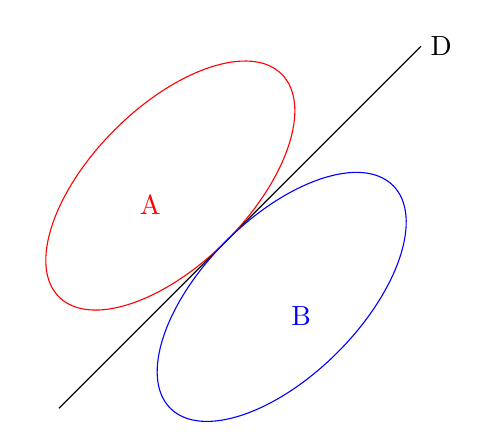
\begin{tikzpicture}
      \begin{scope}[rotate=315]
      \draw (1, -1) -- (1, 5.5) node[right] {D};
      \draw [red] (0 , 2) ellipse (1 cm and 2 cm) node[below left] {A};
      \draw [blue] (2 , 2) ellipse (1 cm and 2 cm) node[below right] {B};
    \end{scope}
    \end{tikzpicture}
\end{center}
\end{figure}

\begin{df}
  Soient $A$, $B$ deux sous-ensembles disjoints de $E$,
  $f:E\to\mathbb{R}$ une forme linéaire continue, $\alpha$ un
  réel et $H = f^{-1}(\{\alpha\})$ un hyperplan affin.

  $H$ sépare $A$ et $B$ au sens large si $\forall x\in A,
  f(x)\leq \alpha$ et $\forall x\in B, f(x)\geq \alpha$.

  $H$ sépare $A$ et $B$ au sens strict s'il existe
  $\varepsilon > 0$ tel que $\forall x\in A, f(x)\leq \alpha
  - \varepsilon$ et $\forall x\in B, f(x)\geq \alpha + \varepsilon$.
\end{df}

Pour parvenir à nos fins, on introduit une fonction appelée jauge
d'un convexe $C$:

\begin{df}
  Soit $C\subseteq E$ un convexe contenant 0 et ouvert.
  Pour tout $x$ dans $E$, on définit la jauge de $C$ en $x$ comme
  suit:
  $$j_C(x) = \inf\left\{\alpha > 0\mid x\in\alpha C\right\}$$
\end{df}

Pour se familiariser avec cette fonction, vous êtes invité
à effectuer les calculs suivants:
\begin{exo}
  On considère le convexe $C = \left]\frac{-1}{2}, 2\right[$.
  Effectuez les calculs suivants:
  \begin{IEEEeqnarray*}{rClCrCl}
    j_C\left(\frac{1}{2}\right) & = & \fbox{\phantom{AAAAAA}}
    &\qquad & j_C\left(-1\right) & = & \fbox{\phantom{AAAAAA}} \\
    j_C\left(\frac{-1}{2}\right) & = & \fbox{\phantom{AAAAAA}}
    &\qquad & j_C\left(2\right) & = & \fbox{\phantom{AAAAAA}} \\
  \end{IEEEeqnarray*}
\end{exo}
